% Exposé VIII. The classification
% Sources: theory/framework.md (Exposé VIII), site/sections/10-atlas.html (#atlas-axes ... #atlas-catalogue),
% theory/axes.json (axes, values, rules, conventions), site/data/atlas-data.js and research/classified/edges.json
% (counts as of the build of 2 October 2026), theory/propositions.json (public statements).
\section{The classification}\label{sec:atlas}

A method is a pointed map $\rho:(Q,q_0)\to(\Theta,\theta_0)$. Its image germ says what it can express
(Exposé~\ref{sec:image}), its fibres and the optimizer's metric how it moves (Exposé~\ref{sec:fibres}), base change what
a moved $\theta_0$ does (Exposé~\ref{sec:base}), and extensions cover adapters and prompts (Exposé~\ref{sec:merge}).
Exposé~\ref{sec:examples} applied this toolkit to fourteen methods. This exposé turns the answers into coordinates and
arrows.

Seven coordinates, each read off the formula, place all \nMethods{} catalogued methods in a periodic table
(Table~\ref{tab:periodic};
\S\ref{sec:atlas-axes} and \S\ref{sec:atlas-table}). Some combinations of coordinates are empty by theorem; for
instance, no linear method starts at an apex. A method $N$ simulates a method $M$ when a pointed smooth map $h$ gives $\rho_N\circ h=\rho_M$.
Five rules produce every arrow, and the atlas records \nArrows{} of them, each with its map $h$; three tests rule arrows
out, and PiSSA and LoRA, for instance, have no arrow either way (\S\ref{sec:atlas-arrows}). Parameters are not reach. At
$131{,}072$ parameters on a $4096\times4096$ matrix, LoRA$_{16}$ reaches $130{,}816$ directions and LoHa$_{8,8}$ at most
$122{,}753$ (\S\ref{sec:atlas-budget}).

\newsavebox{\fbAtlasPeriodicBox}%
\begin{table}[!tbp]
\centering
\caption{The periodic table of the \nCore{} core methods. Rows are kinds (axis~1 of \S\ref{sec:atlas-axes}), with
reparametrisations split by how they couple to $W_0$: additively, by a group action, by a Hadamard product or by
selecting coordinates. Columns are the shapes of the image germ (axis~2). A dot marks an empty cell. All seven
coordinates of the methods named here are in Table~\ref{tab:periodic-methods}, and those of every catalogued method in
Table~\ref{tab:catalogue}.}\label{tab:periodic}
\sbox{\fbAtlasPeriodicBox}{\begin{minipage}{1.3\linewidth}% generated by tools/make_tables.py
\begingroup\scriptsize\setlength{\tabcolsep}{3pt}\renewcommand{\arraystretch}{1.15}
\begin{tabularx}{\linewidth}{@{}>{\raggedright\arraybackslash}p{1.9cm}>{\raggedright\arraybackslash}X>{\raggedright\arraybackslash}X>{\raggedright\arraybackslash}X>{\raggedright\arraybackslash}X>{\raggedright\arraybackslash}X>{\raggedright\arraybackslash}X>{\raggedright\arraybackslash}X@{}}
\toprule\headrow
\textbf{Kind} & \textbf{Lin} & \textbf{Cone} & \textbf{Cone$^{*}$} & \textbf{Orb} & \textbf{Sat} & \textbf{Meet} & \textbf{Fun}\\\midrule
R, additive & C3A, FFA-LoRA, FourierFT, FRoD, InfLoRA, LoRA-FA, LoRA-SB, LoRA-XS, MiCA, MiSS (formerly Bone), MoRA, OSF, SVFT, TinyLoRA, WaveFT & AdaLoRA, AdaMSS, BD-LoRA, DEFT, DeLoRA, DyLoRA, EVA, FacT, GraLoRA, KaSA, KronA, LoHa, LoKr, LongLoRA, LoRA, LoRA+, LoRA-Pro, LoRA-RITE, NOLA, O-LoRA, PEANuT, PVeRA, QA-LoRA, QLoRA, RandLoRA, Riemannian LoRA, RoSA, rsLoRA, Uni-LoRA, VB-LoRA, VeRA & Astra, CorDA, LoftQ, LoRA-GA, LoRETTA, MiLoRA, OLoRA, PiSSA, PRISM & \textcolor{inkgray!70}{\textperiodcentered} & \textcolor{inkgray!70}{\textperiodcentered} & \textcolor{inkgray!70}{\textperiodcentered} & \textcolor{inkgray!70}{\textperiodcentered}\\
R, action & (IA)\textsuperscript{3}, PEQA, RED, SSF & \textcolor{inkgray!70}{\textperiodcentered} & \textcolor{inkgray!70}{\textperiodcentered} & GOFT, LOFT, OFT, OFTv2, Piggyback, qGOFT, RoAd & BOFT, DoRA, PSOFT & HRA, LoCO & \textcolor{inkgray!70}{\textperiodcentered}\\
R, Hadamard & \textcolor{inkgray!70}{\textperiodcentered} & GLoRA, HiRA & \textcolor{inkgray!70}{\textperiodcentered} & \textcolor{inkgray!70}{\textperiodcentered} & \textcolor{inkgray!70}{\textperiodcentered} & \textcolor{inkgray!70}{\textperiodcentered} & \textcolor{inkgray!70}{\textperiodcentered}\\
R, selective & BEFT, BitFit, Child-Tuning, FISH Mask, Linear probing, LN Tuning, LT-SFT, SHiRA, Super-Tuning (Super / Supra), Surgical FT, Trainable Tokens & Diff Pruning & \textcolor{inkgray!70}{\textperiodcentered} & \textcolor{inkgray!70}{\textperiodcentered} & \textcolor{inkgray!70}{\textperiodcentered} & \textcolor{inkgray!70}{\textperiodcentered} & \textcolor{inkgray!70}{\textperiodcentered}\\
E (pointed ext.) & Custom Diffusion, Textual Inversion & \textcolor{inkgray!70}{\textperiodcentered} & \textcolor{inkgray!70}{\textperiodcentered} & \textcolor{inkgray!70}{\textperiodcentered} & \textcolor{inkgray!70}{\textperiodcentered} & \textcolor{inkgray!70}{\textperiodcentered} & Adapter (Houlsby), Compacter, ControlNet, LLaMA-Adapter, LoReFT, Parallel Adapter, Pfeiffer Adapter, ShadowPEFT\\
E$^{0}$ (unpointed) & \textcolor{inkgray!70}{\textperiodcentered} & \textcolor{inkgray!70}{\textperiodcentered} & \textcolor{inkgray!70}{\textperiodcentered} & \textcolor{inkgray!70}{\textperiodcentered} & \textcolor{inkgray!70}{\textperiodcentered} & \textcolor{inkgray!70}{\textperiodcentered} & AutoPrompt, Cartridges, CoOp, CPT, LST, MAM Adapter, MPT, P-Tuning, P-Tuning v2, Prefix-Tuning, Prompt Tuning, UniPELT, VPT\\
B (backward) & Flora, GaLore, LISA, LP-FT, MeZO & ReLoRA & \textcolor{inkgray!70}{\textperiodcentered} & \textcolor{inkgray!70}{\textperiodcentered} & \textcolor{inkgray!70}{\textperiodcentered} & \textcolor{inkgray!70}{\textperiodcentered} & \textcolor{inkgray!70}{\textperiodcentered}\\
P (post hoc) & DARE, Intruder-dimension reduction, KnOTS, LCM-LoRA, LoRA Soups (CAT), Task Arithmetic, TIES-Merging, WiSE-FT & LoraHub & \textcolor{inkgray!70}{\textperiodcentered} & \textcolor{inkgray!70}{\textperiodcentered} & \textcolor{inkgray!70}{\textperiodcentered} & \textcolor{inkgray!70}{\textperiodcentered} & Proxy-Tuning\\
F$_T$ (family) & \textcolor{inkgray!70}{\textperiodcentered} & HyperDreamBooth, Laplace-LoRA, MHR, Polytropon (Poly), Punica, S-LoRA, Text-to-LoRA (T2L) & \textcolor{inkgray!70}{\textperiodcentered} & \textcolor{inkgray!70}{\textperiodcentered} & \textcolor{inkgray!70}{\textperiodcentered} & \textcolor{inkgray!70}{\textperiodcentered} & AdapterFusion, aLoRA, Arrow, HydraLoRA, HyperFormer, Lily, LoRAMoE, MoLE, PHATGOOSE, X-LoRA\\
\bottomrule
\end{tabularx}\endgroup
\end{minipage}}%
\ifdim\dimexpr(\ht\fbAtlasPeriodicBox+\dp\fbAtlasPeriodicBox)*100/130\relax>0.86\textheight
  \resizebox*{!}{0.86\textheight}{\usebox{\fbAtlasPeriodicBox}}%
\else
  \resizebox{\linewidth}{!}{\usebox{\fbAtlasPeriodicBox}}%
\fi
\end{table}

% ------------------------------------------------------------------------------------------------------------------
\subsection{Seven axes, each decidable from the formula}\label{sec:atlas-axes}

\citet{he2021unified} gave adapters four design axes (functional form, insertion form, modified representation and
composition function), and \citet{chen2023parameter} searched a similar design space. The seven axes below extend the
idea to weight-space, backward and post-hoc methods, and each axis is tied to a result.

\makeatletter
\begin{fb@rulebox}[ochre]{1.1pt}\noindent{\normalfont\bfseries\scshape Definition}\ {\normalfont(coordinates of a
method).}\ \upshape
The \emph{coordinates} of a method $M=(Q,q_0,\rho)$ are its answers to the seven questions below, each read off $\rho$,
$q_0$ and the box that $\rho$ acts on, with no training.
\end{fb@rulebox}
\makeatother

The axes and their values are as follows. Table~\ref{tab:axes} states the question each axis asks and defines every
value, Table~\ref{tab:axes-examples} gives the coordinates of LoRA, (IA)$^3$ and prefix tuning, and the ancillary file
\texttt{catalogue.json} repeats the definitions with examples for every value.
\begin{enumerate}[label=\arabic*.]
  \item \textbf{Kind.} R (reparametrisation) $\cdot$ E (pointed extension) $\cdot$ E$^\circ$ (unpointed extension)
  $\cdot$ B (backward lens or schedule) $\cdot$ P (post-hoc operation) $\cdot$ F$_T$ (family over tasks, inputs or
  tenants).
  \item \textbf{Shape} of the image germ. Lin ($\rho$ affine) $\cdot$ Cone (multihomogeneous, non-linear) $\cdot$
  Cone$^*$ (translated cone, split pointing) $\cdot$ Orb (group orbit) $\cdot$ Sat (group $\times$ cone) $\cdot$ Meet
  (orbit $\cap$ cone) $\cdot$ Fun (function level).
  \item \textbf{Base point}, read from $S_1$. regular $\cdot$ apex (deficit $>0$) $\cdot$ neutral $\cdot$ defect
  ($\rho(q_0)\neq\theta_0$) $\cdot$ unpointed.
  \item \textbf{Gauge}, from wire insertions and spider slides, checked by Jacobian rank. none $\cdot$ scalar $\cdot$
  torus $\cdot$ $\GL$ $\cdot$ $\GL\times{}$torus $\cdot$ non-linear.
  \item \textbf{Covariance group} (the Klein geometry of the image). $\GL\times\GL$ $\cdot$ $\CO\times\CO$ $\cdot$
  $\GL\times\CO$ $\cdot$ $\mathrm{Mon}\times\GL$ $\cdot$ $\mathrm{Mon}\times\mathrm{Mon}$ $\cdot$ $\Pi_X$ (imposed
  structure) $\cdot$ frame (random or data, in law).
  \item \textbf{Merge type.} M1 (into its box) $\cdot$ M1$\to$ (into a neighbour via R1--R7, under side conditions)
  $\cdot$ Mq (an exact merge leaves the quantised type) $\cdot$ M$\infty$ (not box-locally mergeable).
  \item \textbf{Rebasing closure.} idempotent $\cdot$ $\to$span $\cdot$ $\to$group $\cdot$ schedule.
\end{enumerate}

\begin{table}[t]
\centering\footnotesize
\caption{The seven questions, answered for three methods. Every answer is read off the formula with no training; the
values of each axis are defined in Table~\ref{tab:axes}.}\label{tab:axes-examples}
\begin{tabularx}{\linewidth}{@{}>{\raggedright\arraybackslash}p{2.0cm}>{\raggedright\arraybackslash}X%
>{\raggedright\arraybackslash}p{2.9cm}>{\raggedright\arraybackslash}p{2.5cm}>{\raggedright\arraybackslash}p{2.25cm}@{}}
\toprule\headrow
\textbf{Axis} & \textbf{Question} & \textbf{LoRA} & \textbf{(IA)$^3$} & \textbf{Prefix tuning}\\\midrule
1\enspace Kind & Where does it act? & R & R & E$^\circ$\\
2\enspace Shape & What is the image germ? & Cone, $d=r(m+n-r)$ & Lin, a torus-orbit closure & Fun\\
3\enspace Base point & Is $\rho(q_0)=\theta_0$? Is $\dim S_1=d(M)$? & apex, deficit $r(n-r)$ & regular & unpointed\\
4\enspace Gauge & Which reparametrisations of $Q$ leave $\rho$ unchanged? & $\GL_r$ & none & non-linear (Li--Liang's
MLP)\\
5\enspace Covariance & For which $(g,h)$ is $\Im M(gW_0h^{-1})=g\,\Im M(W_0)\,h^{-1}$? & $\GL\times\GL$ &
$\mathrm{Mon}\times\GL$; $\GL\times\mathrm{Mon}$ on $W_{\rm down}$ & $\GL\times\GL$, function level\\
6\enspace Merge & Does the update fuse into its box, or by R1--R7 into a neighbour? & M1 & M1$\to$ & M$\infty$\\
7\enspace Rebasing & What does merge-and-restart reach? & $\to$span, all of $\Theta$ at $K=\lceil\min(m,n)/r\rceil$ &
idempotent & --\\
\bottomrule
\end{tabularx}
\end{table}

\subsubsection{Deciding each axis}\label{sec:atlas-decide}

Each axis has a procedure that uses only $\rho$, $q_0$ and the box.
\begin{itemize}
  \item \emph{Kind.} Check whether the trained model is $f(\rho(q),-)$ with the original architecture (R), whether new
  boxes are inserted and some parameter value makes them the identity (E) or none does (E$^\circ$), whether only the
  gradient path or the schedule changes (B), whether the inputs are trained checkpoints (P), and whether the adapter
  depends on a task, an input or a tenant (F$_T$). See \thmref{Definition}{I.2}, \thmref{Definition}{IV.1} and
  \thmref{Definition}{VI.1}.
  \item \emph{Shape.} Read the degree of $\rho-\theta_0$ in $q$. An affine map gives Lin and a multihomogeneous
  non-linear one gives Cone. A group acting on $\theta_0$ gives Orb, a torus acting on another method's image gives Sat
  (\thmref{Proposition}{II.8}), and an intersection gives Meet (\thmref{Theorem}{II.7}).
  \item \emph{Base point.} Evaluate $\rho(q_0)$ and compute $S_1=d\rho_{q_0}(T_{q_0}Q)$, then compare $\dim S_1$ with
  the generic rank $d(M)$ (\thmref{Definition}{I.5}). For LoRA this is \thmref{Theorem}{II.2}(b).
  \item \emph{Gauge.} Insert $gg^{-1}$ on each internal wire between trainable boxes and slide diagonals through copy
  spiders, then confirm $\lvert M\rvert-d(M)$ by a Jacobian rank at a random point
  (\thmref{Proposition}{II.12}(a)).
  \item \emph{Covariance.} Test the identity of \thmref{Definition}{II.14} on generators of $\GL_m\times\GL_n$, in
  distribution when frames are random or come from data.
  \item \emph{Merge.} Run the rewrite rules R1--R7 of \thmref{Theorem}{VI.3} with their side conditions, adding the type
  condition of \thmref{Proposition}{V.2}(d) for a quantised base. The rules are sufficient conditions. They certify M1
  and M1$\to$, and M$\infty$ records a box-local obstruction. Whether a whole network admits some other merge is left
  open.
  \item \emph{Rebasing.} Apply \thmref{Theorem}{V.3}(a) to additive shapes and \thmref{Theorem}{V.3}(b) and (c) to
  actions.
\end{itemize}

\subsubsection{Conventions}\label{sec:atlas-conventions}

\begin{itemize}
  \item \emph{Null coordinates.} ``--'' (null in the classified data) means that the axis does not apply, and no axis
  has a separate ``not applicable'' value. The merge axis keeps a legacy key \texttt{na}, used for backward lenses and
  schedules, which write the full weight directly and so have nothing to merge; it means the same as ``--''.
  \item \emph{When an axis applies.} Shape and gauge need a parameter space, so they are ``--'' for closed-form
  post-hoc operations with no tunable coefficient (Fisher merging without mixing weights, RegMean, uniform model soups),
  which are single points. Base point is ``--'' only for methods with no base point of their own, the serving families
  S-LoRA and Punica. Rebasing needs a weight-space merge, so it is ``--'' for every M$\infty$ method; function-level
  closures belong in the notes. Covariance applies to every method with a formula.
  \item \emph{Function-level covariance.} For extensions and families (shape Fun), covariance is the function-level
  analogue of \thmref{Definition}{II.14}: the inserted or generated family on each adapted wire is invariant under
  conjugation by $(g,h)$ on that wire. Routed mixtures are included, since router and experts transform together.
  \item \emph{Post-hoc operations.} The parameter space of a P operation is its tunable coefficients ($\lambda$ in task
  arithmetic, TIES, DARE, LoRA soups and CAT, LoraHub), and its covariance is the equivariance of the combination rule
  (\thmref{Proposition}{V.4}).
  \item \emph{Nearest keys.} Entries without an exact key are coded to the nearest one: $\CO\times\mathrm{Borel}\to\Pi$
  (OLoRA); $\Ort(r)\to\GL$ (LoReFT, PoLAR); stabiliser $\to$ none (OFT); $\CO(m)\times\GL(n)\to\CO\times\CO$ (Astra,
  whitened splits); $\Ort(m)\times\Ort(n)\to\CO\times\CO$ (LoRA-GA); $\R^\times B_m\times\R^\times B_n\to
  \mathrm{Mon}\times\mathrm{Mon}$ (LoRA-SB); $\R^\times B_N$ and the torus $T_N\to\mathrm{Mon}\times\mathrm{Mon}$ (TIES,
  DARE). One-sided keys ($\mathrm{Mon}\times\GL$, $\GL\times\CO$) name the group up to exchanging the two sides; the
  tables of \S\ref{sec:atlas-table} write (output side) $\times$ (input side).
  \item \emph{Instances.} Arrows and obstructions relate instances of methods: a rank, a pointing, a hyperparameter
  regime. The instance is recorded in the note that accompanies each arrow and obstruction in the ancillary files
  (\S\ref{sec:atlas-checks}).
\end{itemize}

\begin{explains}
Methods with different shapes or base-point types are never isomorphic, however alike their formulas
(\thmref{Observation}{I.4}(c), \thmref{Observation}{I.6}).
\end{explains}

% ---------------------------------------------------- axes table (from theory/axes.json)
\begingroup\footnotesize\setlength{\tabcolsep}{3pt}\renewcommand{\arraystretch}{1.12}
\begin{longtable}{@{}>{\raggedright\arraybackslash}p{2.75cm}>{\raggedright\arraybackslash}p{12.4cm}@{}}
\caption{The seven axes. For each axis, the question it answers and the definition of every value, with the test that
decides it where one is needed. ``--'' (a null coordinate) means that the axis does not apply.}\label{tab:axes}\\
\toprule\headrow\textbf{Value} & \textbf{Definition}\\\midrule
\endfirsthead
\toprule\headrow\textbf{Value} & \textbf{Definition}\\\midrule
\endhead
\bottomrule\endlastfoot
%
\multicolumn{2}{@{}p{\linewidth}@{}}{\textbf{\color{tide}1\enspace Kind} (where the method acts). \emph{Does the method
reparametrise the existing weights, extend the architecture (with or without a neutral point), act only on the backward
pass or the schedule, operate post hoc on several trained points, or form a family over an auxiliary base $T$?}}\\[2pt]
R\newline reparametrisation & A pointed smooth map $\rho:(Q,q_0)\to(\Theta,\theta_0)$ into the existing weight space, an
object of $\Meth(\Theta,\theta_0)=\Diff_*/(\Theta,\theta_0)$. Test: the trained model is $f(\rho(q),-)$ with the
original architecture $f$.\\
E\newline pointed extension & A function-preserving embedding $\iota(\theta)=(\theta,\theta_0')$ into a larger
architecture $\tilde f$ with a neutral point $\theta_0'$, so that $\tilde f(\theta,\theta_0',-)=f(\theta,-)$, followed by a
reparametrisation of $\Theta\times\Theta'$. Test: new boxes are inserted, and some parameter value makes them the
identity.\\
E$^\circ$\newline unpointed extension & An extension with no neutral point: no parameter value reproduces the frozen
function (for prompts and prefixes, \thmref{Theorem}{VI.5}(f) proves this on a head with $W_oW_v\ne0$). Test: try to solve
$\tilde f(\theta_0,p,-)=f(\theta_0,-)$ for $p$.\\
B\newline backward lens or schedule & The forward map is $\id_\Theta$ and the update is
$\theta\leftarrow\theta-\eta\,a_t\big(\mathrm{opt}(c_t(\nabla L))\big)$ with a compression $c_t$ and an anchor $a_t$; or
the method is a sequence of merge-and-restart stages (a rebasing scheme); or it is an optimizer that compresses only its
own state (Flora). Test: the method changes how gradients or optimizer state are compressed, or when the base is
re-pointed, and leaves the parametrisation alone.\\
P\newline post-hoc operation & An operation $\Theta^N\to\Theta$ (or on tuples of factors) applied to several trained
points. Test: the inputs are already-trained adapters or checkpoints.\\
F$_T$\newline family over a base $T$ & A $T$-point $a:T\to Q$ of a method, giving $\rho\circ a:T\to\Theta$, where $T$
is a set of tasks (hypernetworks), the inputs $X$ (routing), a simplex (mixing) or a set of tenants $U$ (serving). Test:
the adapter depends on an auxiliary variable.\\\midrule
%
\multicolumn{2}{@{}p{\linewidth}@{}}{\textbf{\color{tide}2\enspace Shape} of the image germ (expressivity). \emph{What
is the germ at $\theta_0$ of the reachable set $\Im\rho$? Read it from the formula: is $\rho$ affine, multihomogeneous,
a group action, a group acting on a cone, an intersection, or defined only at function level?}}\\[2pt]
Lin\newline linear (flat) & $\rho$ is affine in $q$, so $\Im\rho$ is an affine subspace, and $d(M)$ is the rank of the
linear map, which equals $\lvert M\rvert$ when the map is injective (FourierFT loses one dimension per sampled conjugate
frequency pair). Every point is regular, and rebasing is idempotent when frames, masks and operators are frozen across
cycles.\\
Cone\newline cone with vertex at the start & $\rho-\rho(q_0)$ is multihomogeneous (or a union of linear spaces), and the
image is a non-linear cone with vertex at the start $\rho(q_0)$, which is then a singular point (an apex). The start is
$\theta_0$ for pointed methods, and the quantised or truncated base $\theta_0+e$ for QLoRA-type defects
(\thmref{Proposition}{V.2}). Determinantal, Segre, Hadamard and tensor-network varieties are included.\\
Cone$^*$\newline translated cone (split) & $\rho=\theta_{\rm res}+\delta(q)$ with $\delta$ multihomogeneous and $q_0$
chosen so that $\delta(q_0)=\theta_0-\theta_{\rm res}$ has full rank. The image is a cone whose apex $\theta_{\rm res}$
is not $\theta_0$, and $\theta_0$ is a smooth point (Type II objects).\\
Orb\newline group orbit & $\rho(q)=\gamma(q)\cdot\theta_0$ with $\gamma(q)$ in a group (or monoid) acting linearly on
$\Theta$. Exactly orthogonal actions preserve the Gram matrix and the spectrum. Torus and Hadamard actions keep only the
zeros of $W_0$ (and its row lines while the scales are nonzero), since unconstrained scales can create new zeros.\\
Sat\newline torus saturation & A group or monoid acting on a cone or an orbit: $\Im M=T\cdot\Im N$ for a torus or
diagonal monoid $T$ and a method $N$.\\
Meet\newline meet (pullback) & The image is an intersection of a cone and an orbit (an image-level meet), or the object
is a fibre product of two methods (a categorical product, which exists only when the set-level fibre product is a
manifold).\\
Fun\newline function level & There is no weight-space image: the method lives on an extension and is compared through the
realisation $\Phi_f$.\\\midrule
%
\multicolumn{2}{@{}p{\linewidth}@{}}{\textbf{\color{tide}3\enspace Base point} (the position of $\theta_0$). \emph{Is
$\theta_0=\rho(q_0)$, and if so, is the first-order image $S_1=d\rho_{q_0}(T_{q_0}Q)$ as large as the expressive
dimension $d(M)$?}}\\[2pt]
regular & $\dim S_1=d(M)$, a first-order deficit of $0$: linear methods, orbit methods with an injective orbit map, and
split (Type II) initialisations.\\
apex\newline first-order deficient & $\dim S_1<d(M)$. For cone-shaped germs $\theta_0$ is the vertex. LoRA's deficit is
$r(n-r)$; HRA's paired initialisation has $\dim S_1=kn-k(k+1)/2$ against $d=rn-r(r+1)/2$, with $k=r/2$. DoRA inherits
LoRA's deficit through its torus factor.\\
neutral\newline pointed extension & An extension evaluated at its neutral point: zero up-projection, zero gate, identity
box.\\
defect\newline pointing defect & $\rho(q_0)\neq\theta_0$, by design or by base change; the defect $e=\rho(q_0)-\theta_0$
is part of the data.\\
unpointed & No parameter value reproduces the frozen function.\\\midrule
%
\multicolumn{2}{@{}p{\linewidth}@{}}{\textbf{\color{tide}4\enspace Gauge} (the generic fibre of $\rho$). \emph{Which
transformations of the trainable parameters leave $\rho$ unchanged, and what is the dimension $\lvert M\rvert-d(M)$ of
the generic fibre? Read it off by inserting $gg^{-1}$ on internal wires between trainable boxes and sliding diagonals
through spiders, and confirm it by the generic Jacobian rank.}}\\[2pt]
none\newline trivial & $\rho$ is injective near generic points. There are no charges, and factor-wise operations are
well defined.\\
scalar\newline one scalar slide & A one-parameter group $(b,d)\mapsto(cb,d/c)$ through frozen boxes, with one conserved
charge under gradient flow.\\
torus & A diagonal group (per rank channel or per hidden unit), whose charges are diagonal entries.\\
$\GL$\newline general linear on internal wires & $\GL_r$, or a product of general linear groups on bonds, acting by
$(Bg^{-1},gA)$. The compact half $\so(r)$ gives isometries, and the non-compact half $\Sym_r$ gives $r(r+1)/2$
charges.\\
$\GL\times{}$torus\newline with a Hadamard torus & $\GL$ on each factor plus the torus $(D_1XD_2,D_1^{-1}YD_2^{-1})$
sliding through the copy spider, of dimension $r_1^2+r_2^2+m+n-1$.\\
non-linear & The generic fibre is not an orbit of a linear group action.\\\midrule
%
\multicolumn{2}{@{}p{\linewidth}@{}}{\textbf{\color{tide}5\enspace Covariance group} (the Erlangen geometry of the
image). \emph{For which $(g,h)\in\GL_m\times\GL_n$ does $\Im M(gW_0h^{-1})=g\,\Im M(W_0)\,h^{-1}$ hold for every $W_0$
(in distribution if random frames or data are involved)?}}\\[2pt]
$\GL\times\GL$\newline basis-free & The image transforms with every change of basis on both sides. It satisfies the
sufficient condition of \thmref{Observation}{II.15} for every box-wise linear function-preserving gauge.\\
$\CO\times\CO$\newline spectral frame & The method uses an SVD or another orthogonally equivariant frame of $W_0$, of
gradients or of data. Truncated SVDs are also equivariant under positive scalings, so the group is
$\CO(m)\times\CO(n)=(\R_{>0}\Ort(m))\times(\R_{>0}\Ort(n))$ (\thmref{Proposition}{II.16}). Methods that use bare
singular frames without singular values (LoRA-GA) are scale-invariant rather than covariant and get only
$\Ort(m)\times\Ort(n)$; they are coded with this nearest key.\\
$\GL\times\CO(n)$\newline input-side orthogonal & A right action of $\Ort(n)$ or a subgroup of it. The covariance on the
input side is the normaliser of the structure group: $\CO(n)$ for full OFT, the block normaliser for block OFT.\\
$\mathrm{Mon}\times\GL$\newline one-sided torus & A diagonal torus acts on one side, so only monomial changes of basis
are allowed there.\\
$\mathrm{Mon}\times\mathrm{Mon}$\newline coordinate geometry & Hadamard or support structure in the standard basis on
both sides. It satisfies the sufficient condition of \thmref{Observation}{II.15} for neuron permutations but not for
rotations.\\
$\Pi_X$\newline imposed structure & The method imposes a reshape (a tensor factorisation), a block partition, a cyclic
order or a pairing that the network does not have, and so breaks even neuron permutations (the test of
\thmref{Lemma}{VI.2}).\\
frame\newline random or data frame & Covariance holds only in law, through the distribution of frozen random matrices or
of data statistics.\\\midrule
%
\multicolumn{2}{@{}p{\linewidth}@{}}{\textbf{\color{tide}6\enspace Merge type} (lifting along the realisation).
\emph{After training, does the modified box function stay in the box's function class, and if not, can the rewrite
rules R1--R7 of \thmref{Theorem}{VI.3} (fusion, permutation slide, positive-diagonal slide, spider slide, cup slide, norm
absorption, copy slide) move it into a neighbouring linear box?}}\\[2pt]
M1\newline fuses into its own box & All non-linearity is on the parameter side, and the merge is the canonical map $\rho$
to the terminal object.\\
M1$\to$\newline fuses into a neighbour & A diagonal method merges by R1--R7 into a neighbouring linear box under side
conditions: a position-independent path (under RoPE, scales constant on rotary pairs), an unshared target box (no tying,
and no GQA sharing unless the scale is constant across the group), and a bias slot for shifts. (IA)$^3$ always fuses into
$W_K$, $W_V$ and $W_{\rm down}$; $W_{\rm up}$ is an alternative only under SwiGLU or GeGLU (every scale) or ReLU
(nonnegative scales), and under GELU only for scales in $\{0,1\}$. The rules give sufficient conditions; they do not
decide whole-network mergeability.\\
Mq\newline leaves the quantised type & An exact merge of a generic high-precision update leaves the quantised type (NF4
and recomputed-scale absmax grids are not even closed under addition). Type-preserving merges (dequantise, add and
requantise, as HF PEFT does for bitsandbytes layers) stay on the grid but are lossy. QA-LoRA's group-constant adapters
are the exception.\\
M$\infty$\newline obstructed & The activation side is non-affine in the input for some parameter value (non-linear
adapters, softmax-gated prefixes, input-dependent routing), or the edit acts only at selected positions (ReFT,
position-gated LoRA variants). This is box-local non-mergeability under the rewrite calculus of
\thmref{Theorem}{VI.3}. Whole-network non-mergeability is open, and some residual-stream edits do merge: into an untied
embedding table, a writer's bias or a post-LN affine, or globally for orthogonal edits in RMSNorm models.\\\midrule
%
\multicolumn{2}{@{}p{\linewidth}@{}}{\textbf{\color{tide}7\enspace Rebasing closure} (the reach of merge-and-restart).
\emph{What does the reachable set $R_K=\theta_0+C^{+K}$ (additive) or $R_K=S^K\theta_0$ (action) converge to as the
number $K$ of merge-and-restart cycles grows?}}\\[2pt]
idempotent & The shape is exactly a subspace, subgroup or submonoid independent of the base, with frames, masks and
operators frozen across cycles, so cycles gain nothing (up to closure). Recomputing frames or masks from the merged
weight does gain.\\
$\to$span\newline converges to the span & For a cone closed under real scaling, $R_\infty=\theta_0+\spanop C$. For LoRA,
$R_K=W_0+\MM_{\le\min(Kr,m,n)}$, and full fine-tuning is reached exactly at $K=\lceil\min(m,n)/r\rceil$.\\
$\to$group\newline converges to a generated group & For action methods, $R_\infty$ is the orbit of the monoid generated
by one cycle's image. It is the connected Lie subgroup generated when that image contains a neighbourhood of $e$ in each
generating subgroup (\thmref{Theorem}{V.3}(b)). For block-orthogonal factors it is $\prod_C\SO(C)$ over the connected
components $C$ of the block hypergraph. HF's Cayley--Neumann OFT does not satisfy the hypothesis: for small generators it
generates only a contraction semigroup.\\
schedule\newline a rebasing scheme itself & The method is defined as a sequence of base changes with a moving shape, and
its reach is the sum of the shapes visited.\\
\end{longtable}\endgroup

% ------------------------------------------------------------------------------------------------------------------
\subsection{The periodic table}\label{sec:atlas-table}

Table~\ref{tab:periodic}, at the head of this exposé, places the \nCore{} core methods by kind and by the shape of the image germ, and splits
reparametrisations by how they touch $W_0$: additively, by a group action, by a Hadamard product or by selecting
coordinates. The split refines the additive, selective, reparametrisation-based and hybrid classes of
\citet{lialin2023scaling}; the survey of \citet{han2024parameter} uses a similar split.

Some combinations of coordinates are empty by theorem. An affine $\rho$ has the same differential everywhere, so no linear method
is an apex, and in the catalogue none is. Corollary~2 of \thmref{Theorem}{V.3} ties idempotent rebasing to shapes that
are fixed subspaces, subgroups or submonoids, and of the catalogue's $92$ idempotent methods, $84$ have linear shapes and
$7$ are orbits. The other, WASI \citep{nguyen2025efficient}, trains on the rank-$K$ variety $\MM_{\le K}$ itself, a set
that does not move with the base.

\subsubsection{The table by method}\label{sec:atlas-methods}

Table~\ref{tab:periodic-methods} gives all seven coordinates of the methods the theory works with, together with the
expressive dimension and the maximum rank. In it, $d$ is the expressive dimension, $\rho_{\max}$ the maximum rank, and $k$
(in GraLoRA) the number of blocks per side. ``$\Pi$'' means imposed structure and ``fr'' a random or data frame.
Covariance is written (output side) $\times$ (input side). F$_X$ and F$_U$ are families over inputs and over tenants,
coded F$_T$ in the catalogue, and LoRA$_{(B_0,A_0)}$ is LoRA pointed at $(B_0,A_0)$.

\begingroup\scriptsize\setlength{\tabcolsep}{1.6pt}\renewcommand{\arraystretch}{1.1}%
\newcommand*{\ptn}[1]{\textsuperscript{\sffamily\bfseries\color{tide}#1}}%
\begin{longtable}{@{}>{\raggedright\arraybackslash}p{1.7cm}>{\raggedright\arraybackslash}p{1.5cm}%
>{\raggedright\arraybackslash}p{3.2cm}>{\raggedright\arraybackslash}p{1.6cm}>{\raggedright\arraybackslash}p{1.6cm}%
>{\raggedright\arraybackslash}p{1.75cm}>{\raggedright\arraybackslash}p{1.15cm}>{\raggedright\arraybackslash}p{2.0cm}@{}}
\caption{The periodic table by method: kind, shape (with $d$ and $\rho_{\max}$), base point, gauge, covariance, merge
type and rebasing closure. The notation is explained before the table, and the marks \textdagger, $\approx$ and (fn.)
and the numbered notes after it.}\label{tab:periodic-methods}\\
\toprule\headrow\textbf{Method} & \textbf{Kind} & \textbf{Shape ($d$; $\rho_{\max}$)} & \textbf{Base pt.} &
\textbf{Gauge} & \textbf{Covariance} & \textbf{Merge} & \textbf{Rebasing}\\\midrule
\endfirsthead
\toprule\headrow\textbf{Method} & \textbf{Kind} & \textbf{Shape ($d$; $\rho_{\max}$)} & \textbf{Base pt.} &
\textbf{Gauge} & \textbf{Covariance} & \textbf{Merge} & \textbf{Rebasing}\\\midrule
\endhead
\bottomrule\endlastfoot
Frozen / Full FT & R (initial / terminal) & $\{\theta_0\}$ / $\Theta$ & -- / regular & -- & all / $\GL\times\GL$ & -- &
id\\
LoRA & R & Cone $r(m{+}n{-}r)$; $r$ & apex & $\GL_r$ & $\GL\times\GL$ & M1 & $\to\Theta$ at $K=\lceil\min(m,n)/r\rceil$\\
rsLoRA, LoRA+ & R\ptn{1} & $=$ LoRA & apex & $\GL_r$ & $\GL\times\GL$ & M1 & $\to\Theta$\\
LoRA-Pro, Riem.\ precond., LoRA-RITE & R + metric\ptn{2} & $=$ LoRA & apex & $\GL_r$\ptn{2} & $\GL\times\GL$ & M1 &
$\to\Theta$\\
DeLoRA & R & Cone $\subseteq\Mr$, $\lVert\Delta W\rVert_F\le\lambda\lVert W_0\rVert$ & apex (HF) / split (paper) &
non-linear, fibre $r^2{+}1$\ptn{3} & $\GL\times\GL$ & M1 & $\to\Theta$\\
GraLoRA & R & $\prod$ block cones, $r(m{+}n{-}r)$; $\min(kr,m,n)$ & apex & $\prod\GL_{r/k}$ & $\Pi$ (blocks) & M1 &
$\to\Theta$\\
DyLoRA & R & filtration of cones & apex & $T_r$ & $\GL\times\GL$ & M1 & $\to\Theta$\\
AdaLoRA & R & budgeted union of cones ($P\Lambda Q$) & apex ($\dim S_1=r$) & non-linear, fibre $r(r{+}1)$\ptn{4} &
$\GL\times\GL$ & M1 & $\to\Theta$\\
LoRA-FA (v1/v2) & R & Lin $\{XA_0\}$, $mr$ & regular & none & $\GL\times\mathrm{fr}$ & M1 & id\\
MiSS / Bone & R & Lin $=$ LoRA-FA$(\mathbf 1\T\otimes I_r)$ (balance mode) & regular & none & $\GL\times\Pi$ & M1 &
id\\
MiCA & R & Lin $\{U_{\min}Y\}$ & regular & none & $\CO\times\CO$ & M1 & id\\
LoRA-XS / SVFT / TinyLoRA & R & Lin in SVD frame ($r^2$ / $\lvert\Omega\rvert$ / $u$) & regular (LoRA-XS, TinyLoRA
$\approx$) & none & $\CO\times\CO$ & M1 & id (frames frozen)\\
LoRA-SB & R & Lin $BRA$ in gradient frame, $r^2$ & defect (by design) & none & $\mathrm{Mon}\times\mathrm{Mon}$\ptn{5} &
M1 & id\\
VeRA & R & toric cone, $m{+}r{-}1$; $r$ & apex & $\R^\times$ & $\mathrm{Mon}\times\mathrm{fr}$ & M1 & $\to$
LoRA-FA$(A)$\\
NOLA & R & bilinear cone, $k{+}l{-}1$ & apex & $\R^\times$ & fr & M1 & $\to\spanop\{B_iA_j\}$\\
RandLoRA & R & sum of VeRA-type cones; full rank & apex & torus & fr & M1 & $\to\Theta$\\
VB-LoRA, Uni-LoRA & R & bank / random-tied LoRA images & defect ($\approx$) & discrete & $\Pi$ / fr\ptn{6} & M1 &
$\to\Theta$\\
DoRA & R & Sat $\mathrm{Diag}_m\cdot{}$Cone, $\min(mn,\allowbreak r(m+n-r)+m)$; full & apex & $\GL_r$ &
$\mathrm{Mon}\times\GL$ & M1 & $\to\Theta$\\
PiSSA / MiLoRA & R (Type II) & translated cone & regular (smooth) & $\GL_r$ & $\CO\times\CO$ & M1 & $\to\Theta$\\
OLoRA & R (Type II) & translated cone (QR) & regular (smooth) & $\GL_r$ & $\CO\times\mathrm{Borel}$\ptn{7} & M1 &
$\to\Theta$\\
LoRA-GA / CorDA & R (Type II) & translated cone (gradient / covariance) & regular (smooth) & $\GL_r$ & $\Ort\times\Ort$
/ $\CO\times\CO$ (data)\ptn{8} & M1 & $\to\Theta$\\
Astra & R (Type II) & translated cone (output-activation second moment) & regular (smooth) & $\GL_r$ & $\CO\times\GL$
(data)\ptn{9} & M1 & $\to\Theta$\\
EVA & R (Type I) & $=$ LoRA\ptn{10} & apex & $\GL_r$ & $\GL\times\GL$\ptn{10} & M1 & $\to\Theta$\\
QLoRA & R at $\kappa\theta_0$ & cone at $\kappa\theta_0$ & defect $e$ & $\GL_r$ & Mon (grid) & Mq & $\to\Theta$\\
LoftQ & R (approx.\ Type II) & translated cone over a quantised residual & defect\ptn{11} & $\GL_r$ & Mon & Mq &
$\to\Theta$\\
LoHa & R & Hadamard variety, $\le\min(mn,\allowbreak 2r(m+n)-2r^2-(m+n-1))$; $\min(r^2,m,n)$ & apex & $\GL_r^2\times{}$torus
& $\mathrm{Mon}\times\mathrm{Mon}$ & M1 & $\to\Theta$\\
LoKr / KronA & R & $\mathcal R^{-1}$-transported cone; $\rk C\cdot r'$ & apex & $\R^\times(\times\GL_{r'})$ &
$\Pi_\otimes$ & M1 & $\to\Theta$\\
TT / Tucker (FacT, LoTR; LoRETTA) & R & meet of transported cones\ptn{12} & apex / regular\ptn{12} & $\prod\GL_{r_e}$ &
$\Pi_\otimes$ & M1 & $\to\Theta$\\
MoRA & R & Lin, $\hat r^2$; high rank & regular & none & $\Pi$ (blocks) & M1 & id (fixed operators)\\
HiRA & R & $(D_{W_0})_*$Cone; $r\rk W_0$ & apex & $\GL_r$ & $\mathrm{Mon}\times\mathrm{Mon}$ & M1 & $\to\Theta$ (not
transported ReLoRA)\\
FourierFT / WaveFT & R & Lin (sparse in the real Fourier / wavelet frame) & regular\ptn{13} & none\ptn{13} &
$\Pi_{\rm cyc}$ / $\Pi$ & M1 & id (fixed indices)\\
C3A & R & Lin (block-circulant), $mn/b$; full & regular & none & $\Pi_{\rm cyc}$ & M1 & id\\
SHiRA / FISH & R & Lin (fixed coordinate mask) & regular & none & $\mathrm{Mon}\times\mathrm{Mon}$ & M1 & id\\
Trainable Tokens & R & Lin (fixed row mask on the embedding and a tied head) & regular & none &
$\GL\times\mathrm{Mon}$\ptn{14} & M1 & id\\
Diff pruning & R & $\bigcup$ $k$-sparse subspaces & apex & none & $\mathrm{Mon}\times\mathrm{Mon}$ & M1 & $\to\Theta$\\
BitFit / LN-tuning & R & Lin (bias / LN parameters) & regular & none & $\GL\times\GL$ / Mon & M1 / M1$\to$ & id\\
OFT (block) & R & Orb of $\prod\SO(b)$ (exact Cayley); quasi-orthogonal (HF)\ptn{15} & regular & stabiliser\ptn{15} &
$\GL\times N_{\rm blk}$ & M1 & id up to closure (exact); $K_{\rm out}$ shrinks (HF)\ptn{15}\\
BOFT (HF) & R & $\diag(\R^m)\times{}$butterfly product & regular\textdagger & inter-factor & $\mathrm{Mon}\times\Pi$ & M1
& $\to\diag\cdot W_0\cdot{}$\hspace{0pt}$\prod\SO(b\,2^{m'-1})$; $\SO(n)$ only at full depth\\
GOFT (strict) / qGOFT & R & Givens product / free $2\times2$ blocks\ptn{16} & regular & none / torus\ptn{16} &
$\GL\times\Pi$ & M1 & $\to W_0\SO(n)$ / $W_0\R^{n\times n}$\ptn{16}\\
HRA & R & Meet $(W_0{+}\Mr)\cap W_0\SO(n)$ (image level), $rn-\tfrac{r(r+1)}2$ & \textbf{apex} & non-linear, fibre
$\tfrac{r(r+1)}2$ & $\GL\times\CO$ & M1 & $\to W_0\SO(n)$ in $\lceil n/r\rceil$\\
(IA)$^3$ / SSF / RED & R & Lin $=$ closure of a torus orbit & regular & none & $\mathrm{Mon}\times\GL$ /
$\GL\times\mathrm{Mon}$\ptn{17} & M1$\to$ & id\\
RoAd & R & RoAd$_1$: orbit closure of $(\mathbb C^\times)^{m/2}$, $m$; RoAd$_{2,4}$: Lin, $2m$ & regular & none
(RoAd$_4$: per block) & $\mathrm{Mon}_{\rm pair}\times\GL$ & M1 & id\\
Houlsby / Pfeiffer & E & Fun (serial, non-linear) & neutral\ptn{18} & $S_r$ / $S_r\ltimes\R_{>0}^r$\ptn{18} &
$\GL\times\GL$ (fn.) & M$\infty$ & --\\
Parallel adapter & E & Fun\ptn{19} & neutral & $S_r\ltimes\R^r_{>0}$\ptn{19} & $\GL\times\GL$ (fn.) & M$\infty$\ptn{19}
& --\\
Compacter & E & Fun with PHM weights\ptn{20} & neutral & torus\ptn{20} & $\Pi_\otimes$ & M$\infty$ & --\\
LST & E$^\circ$ & Fun (side network)\ptn{21} & unpointed\ptn{21} & $\GL$ (side network) & $\GL\times\GL$ (fn.) &
M$\infty$ & --\\
LLaMA-Adapter & E & Fun (separately normalised prefix) & neutral ($g=0$) & none & $\GL\times\GL$ (fn.) & M$\infty$ &
--\\
LoReFT & E\ptn{22} & LoRA$_r$ on $\mathrm{Aff}(I_d)$, $r(2d{+}1{-}r)$ & defect\ptn{22} & $\Ort(r)$\ptn{22} &
$\GL\times\GL$ (fn.) & M$\infty$ & --\\
Prompt tuning / P-tuning v1 & E$^\circ$ & Fun (input state)\ptn{23} & unpointed & none / non-linear\ptn{23} &
$\GL\times\GL$ (fn.) & M$\infty$ & --\\
Prefix / P-tuning v2 & E$^\circ$ & Fun (gated parallel adapter, per layer) & unpointed & non-linear / none\ptn{24} &
$\GL\times\GL$ (fn.) & M$\infty$ & --\\
MPT / CPT & E$^\circ$ & $P^*\odot uv\T$ / ball\ptn{25} & unpointed / pointed\ptn{25} & torus / none\ptn{25} &
$\GL\times\GL$ / $\CO\times\CO$ (fn.) & M$\infty$ & --\\
GaLore & B & moving Lin $\{P_tX\}$ & regular & none & $\CO\times\CO$ (gradient) & -- & $\to\Theta$\\
GaLore with a random projector & B & moving Lin $\{XA_t\}$ & regular & none & fr & -- & $\to\Theta$\\
Flora & B\ptn{26} & Lin $=\Theta$\ptn{26} & regular & none & fr (in law)\ptn{26} & -- & --\\
LISA & B & moving layer blocks & regular & none & $\GL\times\GL$\ptn{27} & -- & $\to\Theta$\\
MeZO & B & moving random line & regular & none & $\Ort(\Theta)$ in law & -- & $\to\Theta$\\
ReLoRA & B & cone per stage $\to\MM_{\le Kr}$ & apex per stage & $\GL_r$ per stage & $\GL\times\GL$ & M1 & schedule\\
Task arithmetic & P & Lin $\theta_0+\sum\lambda_i\tau_i$ & regular ($\lambda=0$) & none & $\GL(\Theta)$ & M1 & id\\
TIES / DARE & P & Lin in $\lambda$ (coordinatewise rule) & regular & none & $\R^\times\cdot B_N$ /
$\mathrm{Mon}_N$\ptn{28} & M1 & id\\
LoRA soups / CAT & P & $\oplus$ of frozen line methods\ptn{29} & regular & none & $\GL\times\GL$ & M1 & id\\
LoraHub / Poly / MHR & P / F$_T$ & factor-wise product of sums & apex & $\prod\GL_r$, broken by LoraHub\ptn{30} &
$\GL\times\GL$ / $\Pi$\ptn{30} & M1 per task & --\\
MoLE / LoRAMoE / X-LoRA & F$_X$ & input-dependent mixture & neutral / unpointed\ptn{31} & per expert / scalar /
none\ptn{31} & $\GL\times\GL$ (fn.)\ptn{31} & M$\infty$\ptn{31} & --\\
S-LoRA / Punica & F$_U$ & LoRA cone per tenant over a shared base & -- & $\prod_u\GL_{r_u}$ & $\GL\times\GL$ & M1 per
tenant\ptn{32} & --\\
Text-to-LoRA / HyperFormer & F$_T$ & a $T$-point of LoRA / of non-linear adapters & apex / defect\ptn{33} & $\GL_r$ /
$\GL$\ptn{33} & $\GL\times\GL$ & M1 / M$\infty$\ptn{33} & --\\
UniPELT / MAM & E$^\circ$\ptn{34} & Fun, not a $\oplus$-word\ptn{34} & unpointed\ptn{34} & $\GL$\ptn{34} &
$\GL\times\GL$ (fn.) & M$\infty$\ptn{34} & --\\
\end{longtable}\endgroup

\paragraph{Notes on the table}
\textdagger\ BOFT's identity is regular when the factors' plane sets are disjoint (for example $b=2$), because then the
factor Lie algebras form a direct sum. ``$\approx$'' marks implementations whose default initialisation is near, but not
exactly at, $\theta_0$: the FourierFT and C3A defaults in HF PEFT, VB-LoRA, Uni-LoRA, TinyLoRA, and LoRA-XS
($R_0\sim\mathcal N(0,10^{-10})$). They are objects of the unpointed slice with a pointing defect, small for LoRA-XS and
TinyLoRA but not for HF's FourierFT ($\mathcal N(0,1)$ spectrum with scaling $150$, about $14\%$ of a std-$0.04$ $W_0$
at $768^2$ with $1000$ frequencies), and the table classifies their exactly pointed variants. ``$\CO\times\CO$'': frames
built from truncated SVDs are equivariant under positive scalings as well as orthogonal maps, so the spectral-frame
geometry is $\CO(m)\times\CO(n)$ (\thmref{Proposition}{II.16}); bare singular frames used without their singular values
(LoRA-GA) are scale-invariant rather than covariant, which leaves $\Ort(m)\times\Ort(n)$. ``(fn.)'' marks the
function-level analogue of \thmref{Definition}{II.14}: the inserted or generated family on each adapted wire is
invariant under conjugation by $(g,h)$ on that wire. ``--'' means that the axis does not apply (null in the classified
data). Where the classified data refines an entry (Kind, Gauge, Covariance and Merge of LST, UniPELT and MAM, MPT,
Compacter, Houlsby, DeLoRA, AdaLoRA, LoRETTA, LoRA-SB, Trainable Tokens, VB-LoRA, LISA, HyperFormer, S-LoRA and Punica),
the table follows the data.

Dimensions hold under the hypotheses of the results that compute them. HRA's is for $W_0$ of full column rank and even
$r\le n-2$ (\thmref{Theorem}{II.7}); DoRA's is for generic $W_0$ with no zero rows, and it drops for special $W_0$
(\thmref{Proposition}{II.8}); GraLoRA's is for HF's default \texttt{hybrid\_r=0} (\thmref{Proposition}{II.12}); and
LoHa's entry is an upper bound, with equality checked numerically below the $mn$ cap (\thmref{Proposition}{II.12}).

\paragraph{Notes by row}
The superscript numbers in Table~\ref{tab:periodic-methods} refer to these notes.
{\small
\begin{enumerate}[label={\sffamily\bfseries\color{tide}\arabic*},leftmargin=1.6em,itemsep=1pt,topsep=3pt]
  \item rsLoRA and LoRA+ are LoRA up to the hyperparameter torus.
  \item LoRA-Pro, Riemannian preconditioning and LoRA-RITE are reparametrisations with a descending metric (their SGD
  forms). The $\GL_r$ gauge is respected only undamped; LoRA-Pro's parameter step keeps $\Ort(r)$, and LoRA-RITE keeps
  $\GL_r$ on the full-rank locus (\thmref{Theorem}{III.12}).
  \item DeLoRA: its per-term scalings form a $2r$-torus inside the fibre; for $r=1$ the fibre is that torus.
  \item AdaLoRA: the fibre consists of two torus edges and the absorption of $\Lambda$.
  \item LoRA-SB: the covariance is $\R^\times B_m\times\R^\times B_n$, because the frame is the SVD of a sign-gradient.
  \item VB-LoRA: $\Pi$, the chunk partition tied across boxes by the shared bank. Uni-LoRA: a random frame.
  \item OLoRA: the QR frame makes the input side Borel. The catalogue key is $\Pi$, since the order of the inputs
  matters.
  \item LoRA-GA: $\Ort\times\Ort$, from data; its bare singular frames are scale-invariant and depend on the sign
  convention. CorDA: $\CO\times\CO$, from data, at the level of the formula.
  \item Astra: the split is $\Phi(W_0CW_0\T)W_0$ (\thmref{Proposition}{II.16}).
  \item EVA is LoRA with $\mathrm{row}\,A_0$ spanned by principal components of the activations. Its covariance is
  $\GL\times\GL$ at a fixed rank (frame $\CO$), and $\GL\times\CO$ with HF's default \texttt{rho=2}.
  \item LoftQ: the defect is the attained residual when $s=1$; HF ignores the scale $s=\alpha/r$.
  \item TT and Tucker methods sit at the apex for zero-core initialisations. LoRETTA's compensated split initialisation
  is regular, and its shape is a meet of translated cones (Cone$^*$).
  \item FourierFT and WaveFT are regular with \texttt{init\_\allowbreak weights=True}; HF's FourierFT default is a
  defect ($\approx$). The gauge gains one dimension for each sampled conjugate pair.
  \item Trainable Tokens: $\GL$ on the embedding dimensions, Mon on the vocabulary.
  \item OFT: with the exact Cayley map the shape is the orbit of $\prod\SO(b)$ in the level set of $K_{\rm out}$, and
  rebasing is the identity up to closure. HF's default Cayley--Neumann map is only quasi-orthogonal, and its merges
  shrink $K_{\rm out}$ monotonically when $\lVert Q\rVert_{\rm op}\le2^{1/4}$. The gauge is the stabiliser of $W_0$,
  trivial for injective $W_0$; the catalogue key is ``none''.
  \item GOFT and qGOFT: qGOFT replaces each Givens rotation by an arbitrary $2\times2$ block, and its gauge is a torus of
  dimension $d-2$. GOFT's official code adds an input scaler by default (\thmref{Corollary}{II.6}), and the row is for
  strict GOFT. When the planes connect all coordinates, as in GOFT's layout, re-merging reaches $W_0\SO(n)$ for GOFT.
  For qGOFT it reaches $W_0\R^{n\times n}$, the matrices whose columns lie in $\operatorname{col}W_0$: its blocks
  include singular ones and ones of negative determinant, and on connected planes they generate the monoid of all
  $n\times n$ matrices (\thmref{Theorem}{V.3}(b)).
  \item (IA)$^3$, SSF and RED: $\mathrm{Mon}\times\GL$ for output scalings, $\GL\times\mathrm{Mon}$ for scaling
  $W_{\rm down}$.
  \item Houlsby and Pfeiffer adapters are neutral with a zero up-projection; Houlsby's own near-identity initialisation
  leaves a small defect. Houlsby's gauge is only $S_r$ (GELU in the reference code, swish in AdapterHub); Pfeiffer's is
  $S_r\ltimes\R_{>0}^r$ (ReLU).
  \item A parallel adapter with $\sigma=\id$, parallel to one linear box, is LoRA and merges as M1. The gauge
  $S_r\ltimes\R^r_{>0}$ is for ReLU, as in the code of He et al.
  \item Compacter: the PHM weights are Kronecker-structured and shared. The torus consists of per-term slides; a $\GL$
  mixing of the PHM index leaves the rank-$\rho$ class.
  \item LST: the side network is fed through trainable down-projection ladders. The up-projection has rank at most
  $d/r$, so no parameter value reproduces $f$.
  \item LoReFT is an extension at an affine identity box over positions. The pyreft initialisation leaves a defect;
  LoReFT is neutral iff $W=R$ and $b=0$. The catalogue key for its gauge is $\GL$.
  \item Prompt tuning has no gauge. P-tuning v1 adds an LSTM or MLP 2-cell, and its gauge is non-linear, through that
  encoder.
  \item Prefix tuning has a non-linear gauge through the MLP of Li and Liang; P-tuning v2 trains the prefix directly and
  has none.
  \item MPT's prompt is $P^*\odot uv\T$, and MPT is unpointed. CPT's prompt lies in a ball around the demonstrations and
  is pointed at the in-context-learning context. MPT's gauge is a torus of dimension $\ell+d$ with $P^*$ trainable
  ($\R^\times$ with $P^*$ frozen); CPT has none.
  \item Flora compresses only its momentum and takes full-space Adafactor steps (\thmref{Proposition}{IV.2}); its random
  frame is the momentum projection, in law.
  \item LISA: each stage frees whole boxes.
  \item TIES elects signs by total mass, and its covariance is $\R^\times\cdot B_N$. DARE's is $\mathrm{Mon}_N$: the
  torus exactly for each mask, the permutations in law.
  \item CAT is a $\oplus$ of frozen line methods, $\spanop\{B_iA_i\}$ per layer, inside LoRA$_{kr}$.
  \item LoraHub, which combines adapters post hoc, is gauge-dependent and breaks $\prod\GL_r$; Poly and MHR, trained
  jointly, keep a diagonal $\GL_r$. The covariance is $\GL\times\GL$ on LoraHub's products and $\Pi$ (blocks) for MHR.
  \item LoRAMoE is neutral, MoLE and X-LoRA are unpointed. The gauge is $\GL_r$ per expert for LoRAMoE, a scalar for
  MoLE (only the gate trains) and none for X-LoRA (only the head trains). Router and experts transform together.
  Merging is M1 when the gate is constant.
  \item S-LoRA and Punica compute relative to a shared base, and each tenant's fibre is a LoRA cone. Each tenant is
  left unmerged by design, to share the base batch.
  \item Text-to-LoRA is at the apex; HyperFormer's random hypernetworks leave a defect. The gauge is $\GL_r$ on the
  generated rank wire for Text-to-LoRA and $\GL$ on the task-embedding wire for HyperFormer, and factor targets are
  gauge-sensitive. Merging is M1 per task for Text-to-LoRA and M$\infty$ for HyperFormer.
  \item UniPELT's gates also make it an F$_X$. Its adapter and prefix parts sit on extensions, so it is not a
  $\oplus$-word. It is unpointed: the prefix has no neutral value, and UniPELT's gate scales the prefix keys rather
  than their softmax mass. The $\GL$ gauge comes from UniPELT's LoRA summand and MAM's prefix MLP. Merging is M$\infty$,
  also for UniPELT's input-gated LoRA part.
\end{enumerate}}

\subsubsection{Checks on the table}\label{sec:atlas-checks}

Several entries rest on numerical checks reported in Appendix~\ref{app:repro}: the GraLoRA and LoHa dimensions and the
LoHa orbit, the HRA apex (by the Jacobian rank at the paired initialisation), the RoAd orbit dimension, the VeRA rebasing
span, the DoRA dimension caps, the FourierFT conjugate pairs, the LoraHub and Poly fibres, and the Cayley--Neumann
contraction [Num].

The classified data pass the following structural checks. Every arrow and every obstruction joins two catalogued
methods and names a valid rule or test. A check at the level of method identifiers flags $26$ pairs that carry both an
arrow and an obstruction, and $8$ arrows from a method to itself. Each flagged pair concerns two instances of the
target: a different rank, pointing, hyperparameter regime or variant. For example, PiSSA$_r$ maps into LoRA$_{2r}$ at the
degenerate pointing with product $0$ (\thmref{Theorem}{II.1}), while the O3 obstruction concerns LoRA$_r$ at its apex,
whose image is incomparable with PiSSA's (\thmref{Theorem}{II.2}(d)). Each self-arrow is an inclusion between instances
of one family, such as LoRA$_r\hookrightarrow{}$LoRA$_{r+1}$, ReLoRA$^K\hookrightarrow{}$ReLoRA$^{K+1}$ or BOFT with
$m'$ butterfly factors inside BOFT with $m'+1$.

The data deviate from the conventions of \S\ref{sec:atlas-conventions} in eight recorded places, which are kept as
published in the ancillary files.
\begin{enumerate}[label=(\arabic*)]
  \item Sixteen function-level families and post-hoc compositions carry no covariance (LoRAMoE, MixLoRA, HydraLoRA,
  ICEdit, MoV, Lily, MoLE, X-LoRA, PHATGOOSE, Arrow, LoraRetriever, LoRA-Flow, SMEAR, GOAT, AdapterSoup and LoRA
  Switch). Under the conventions they carry their expert family's function-level value: $\GL\times\GL$ for dense LoRA
  experts and routers, and $\mathrm{Mon}\times\GL$ for MoV.
  \item Initial-state tuning and state-offset tuning are M$\infty$ with rebasing ``idempotent''; under the conventions
  their rebasing is ``--''.
  \item Flora is coded as a per-period linear method with rebasing ``schedule''. Flora takes full-space steps and
  compresses only its momentum (\thmref{Proposition}{IV.2}), so its per-step shape is all of $\Theta$ and its rebasing
  is ``--'', as in Table~\ref{tab:periodic-methods}.
  \item EVA is coded $\GL\times\GL$, which holds at a fixed rank; HF's default \texttt{rho=2} gives $\GL\times\CO(n)$
  (\thmref{Proposition}{II.16}).
  \item OFTv2's rebasing note says that its Cayley--Neumann factors generate $\prod\GL^+(b)$ and that $K_{\rm out}$
  drifts. \thmref{Theorem}{V.3} gives a contraction semigroup, with monotone shrinkage of $K_{\rm out}$, for small
  generators.
  \item Fisher merging's optional mixing weights would make it a coefficient family under the post-hoc convention.
  \item The entries MoV / MoLoRA and Child-Tuning (its D and F variants) each cover two variants.
  \item The ``core'' flag is not a coordinate. It marks every method named in Table~\ref{tab:periodic-methods} plus a
  curated set.
\end{enumerate}

\subsubsection{The whole catalogue}\label{sec:atlas-catalogue}

Everything above rests on a catalogue of \nMethods{} methods and \nPapers{} papers, checked against arXiv and, for
library claims, against Hugging Face PEFT \citep{xmangrulkar2022peft} as of 30 September 2026; \nHF{} of the methods
ship in that library. Each method entry gives the formula, budget, locus, kind, merge verdict, initialisation, relations,
sources, coordinates and a categorical reading, most with arrows and obstructions. Appendix~\ref{app:catalogue} lists
every method with its seven coordinates and its reference (Table~\ref{tab:catalogue}) and every arrow with its map $h$
(Table~\ref{tab:arrows}); the ancillary files \texttt{catalogue.csv}, \texttt{arrows.csv} and
\texttt{obstructions.csv} carry the full entries. Table~\ref{tab:atlas-counts} counts the methods per coordinate value.
Cones and linear shapes account for $240$ of the \nMethods{} methods, and apex and regular base points are about equally
common.

Earlier maps made this one possible: the surveys of \citet{lialin2023scaling}, \citet{xu2023parameter},
\citet{han2024parameter} and \citet{mao2024survey}, the delta-tuning study of \citet{ding2022parameter}, and the
libraries AdapterHub \citep{pfeiffer2020adapterhub}, Adapters \citep{poth2023adapters} and Hugging Face PEFT
\citep{xmangrulkar2022peft}, whose source settled many details.

\begin{table}[t]
\centering\footnotesize
\caption{The classification of all \nMethods{} catalogued methods: the number of methods with each coordinate value,
over all methods / over the \nCore{} core methods. ``--'' counts null coordinates, including the legacy merge key
\texttt{na}. Per-method values are in Table~\ref{tab:catalogue}.}\label{tab:atlas-counts}
\begin{tabularx}{\linewidth}{@{}>{\raggedright\arraybackslash}p{1.9cm}>{\raggedright\arraybackslash}X@{}}
\toprule\headrow
\textbf{Axis} & \textbf{Value: all / core}\\\midrule
Kind & R $208/85$ $\cdot$ E $33/10$ $\cdot$ E$^\circ$ $27/13$ $\cdot$ B $29/6$ $\cdot$ P $31/11$ $\cdot$ F$_T$ $54/17$\\
Shape & Lin $106/45$ $\cdot$ Cone $134/43$ $\cdot$ Cone$^*$ $20/9$ $\cdot$ Orb $13/7$ $\cdot$ Sat $5/3$ $\cdot$ Meet
$2/2$ $\cdot$ Fun $93/32$ $\cdot$ -- $9/1$\\
Base point & regular $113/56$ $\cdot$ apex $111/40$ $\cdot$ neutral $40/13$ $\cdot$ defect $59/13$ $\cdot$ unpointed
$57/18$ $\cdot$ -- $2/2$\\
Gauge & none $139/62$ $\cdot$ scalar $9/6$ $\cdot$ torus $40/9$ $\cdot$ $\GL$ $152/51$ $\cdot$ $\GL\times{}$torus $3/1$
$\cdot$ non-linear $23/10$ $\cdot$ -- $16/3$\\
Covariance & $\GL\times\GL$ $166/53$ $\cdot$ $\CO\times\CO$ $47/20$ $\cdot$ $\GL\times\CO$ $12/5$ $\cdot$
$\mathrm{Mon}\times\GL$ $21/10$ $\cdot$ $\mathrm{Mon}\times\mathrm{Mon}$ $52/18$ $\cdot$ $\Pi$ $49/19$ $\cdot$ frame
$19/10$ $\cdot$ -- $16/7$\\
Merge & M1 $242/98$ $\cdot$ M1$\to$ $11/5$ $\cdot$ Mq $11/2$ $\cdot$ M$\infty$ $97/32$ $\cdot$ -- $21/5$\\
Rebasing & idempotent $92/43$ $\cdot$ $\to$span $130/45$ $\cdot$ $\to$group $12/7$ $\cdot$ schedule $29/9$ $\cdot$ --
$119/38$\\
\bottomrule
\end{tabularx}
\end{table}

Figure~\ref{fig:timeline} dates each method by its first arXiv submission. Landmarks come in rough order, with
bottleneck adapters in 2019 \citep{houlsby2019parameter}, prefixes \citep{li2021prefix} and LoRA's cone
\citep{hu2021lora} in 2021, the torus of (IA)$^3$ in 2022 \citep{liu2022few}, base change with QLoRA in 2023
\citep{dettmers2023qlora}, and GaLore's moving frame in 2024 \citep{zhao2024galore}, the year of $113$ of the
\nMethods{} methods.

\begin{figure}[tbp]
\centering
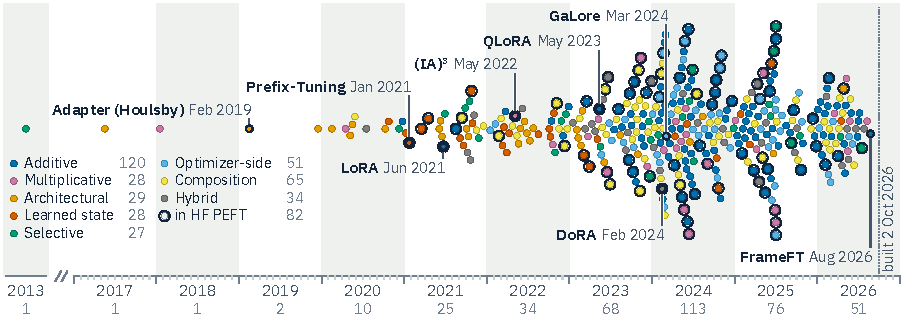
\includegraphics[width=\linewidth]{figures/timeline}
\caption{\textbf{The catalogue in time.} Each of the \nMethods{} catalogued methods is one dot, placed at the month of its paper's first arXiv submission, read from the YYMM prefix of its identifier; within a month the dots are spread evenly in the order of their arXiv numbers, and the six entries without an identifier sit at mid-year. The dots form a centred beeswarm, coloured by modification kind (legend, with the number of entries of each kind) and ringed when the method ships in Hugging Face PEFT (\nHF{} entries). The one entry before 2017, linear probing on DeCAF features \citep{donahue2013decaf}, sits left of the axis break. The number under each year counts its entries, from $10$ in 2020 to $113$ in 2024; the busiest month is February 2024, with $20$. The 2026 count ends at the catalogue's build date, 2~October~2026 (dotted line). Labels mark the bottleneck adapter \citep{houlsby2019parameter}, prefix tuning \citep{li2021prefix}, LoRA \citep{hu2021lora}, (IA)$^3$ \citep{liu2022few}, QLoRA \citep{dettmers2023qlora}, DoRA \citep{liu2024dora}, GaLore \citep{zhao2024galore} and the newest entry, FrameFT \citep{adepu2026fine}. Additive weight edits are the largest kind ($120$ entries), followed by composition and routing ($65$) and optimizer-side methods ($51$).}\label{fig:timeline}
\end{figure}

\subsubsection{What a budget buys}\label{sec:atlas-budget}

\thmref{Proposition}{II.12} separates the budget $\lvert M\rvert$, what a method trains, from the expressive dimension
$d(M)$, the number of directions in which it can move the weights. The gap is gauge waste (\thmref{Definition}{I.5}): per
matrix, $r^2$ for LoRA, one for VeRA (numerically), zero for injective linear methods, and at least $2r^2+m+n-1$ for
LoHa$_{r,r}$ (\thmref{Proposition}{II.12}). At $131{,}072$ parameters on a $4096\times4096$ matrix, LoRA$_{16}$ reaches
$130{,}816$ directions at rank up to $16$, and LoHa$_{8,8}$ at most $122{,}753$ at rank up to $64$. Rankings at matched
budget and at matched $d(M)$ can differ (\thmref{Prediction}{X.10}). Figure~\ref{fig:rankvol} compares maximum rank and
$d(M)$ at equal budget for eight methods on such a layer, and the companion site's budget calculator computes both counts
for the adapted matrices of common base models.

% ------------------------------------------------------------------------------------------------------------------
\subsection{Arrow rules: when \texorpdfstring{$N$}{N} simulates \texorpdfstring{$M$}{M}}\label{sec:atlas-arrows}

``Generalises'' and ``is a special case of'' get one reading here. $N$ simulates $M$ when a pointed smooth map
$h:Q_M\to Q_N$ satisfies $\rho_N\circ h=\rho_M$ (\thmref{Definition}{I.2}), so $N$ reaches every weight that $M$
reaches. A morphism $M\to N$ is exhibited by an explicit pointed $h$. Five rules generate every arrow in the atlas, and
three tests rule arrows out (Table~\ref{tab:atlas-rules}).

\begin{table}[t]
\centering\footnotesize
\caption{The arrow rules A1--A5, transport T and the obstruction tests O1--O3. An arrow $M\to N$ is a pointed smooth
map $h:Q_M\to Q_N$ with $\rho_N\circ h=\rho_M$.}\label{tab:atlas-rules}
\begin{tabularx}{\linewidth}{@{}>{\raggedright\arraybackslash}p{1.8cm}>{\raggedright\arraybackslash}X%
>{\raggedright\arraybackslash}p{3.65cm}>{\raggedright\arraybackslash}p{4.5cm}@{}}
\toprule\headrow
\textbf{Rule} & \textbf{Statement} & \textbf{The map $h$, or the test} & \textbf{Examples}\\\midrule
\textbf{A1}\newline interval & Frozen${}\to M\to{}$Full FT for every weight-space $M$. & $h=\mathrm{const}_{q_0}$; $h=\rho_M$ &
Merging is the arrow to Full FT.\\
\textbf{A2}\newline freezing & Freezing coordinates at their base values gives a sub-object. & $h(q')=(q',q_0'')$ &
$\mathrm{FA}(A_0)\hookrightarrow{}$LoRA pointed at $(0,A_0)$; MiCA${}\hookrightarrow{}$LoRA pointed at $(B_0,0)$.\\
\textbf{A3}\newline factorisation & $\rho_M=\rho_N\circ h$ for an explicit pointed map $h$, usually polynomial. & VeRA${}\to
\mathrm{FA}(A)$: $h(b,d)=\Lambda_bB\Lambda_d$. LoHa$_{r_1,r_2}\to{}$LoRA$_{r_1r_2}$: face-splitting products.
(IA)$^3\to{}$HiRA$_1$ pointed at $(0,\mathbf 1\T)$: $h(\ell)=(\ell-\mathbf 1,\mathbf 1\T)$. & Isomorphisms:
rsLoRA${}\cong{}$LoRA by $h=(\sqrt r\,B,A)$; MiSS (balance mode) ${}\cong\mathrm{FA}(\mathbf 1\T\otimes I_r)$; a linear
adapter parallel to one layer ${}\cong{}$LoRA.\\
\textbf{A4}\newline products & A product comes with its two projections. & $R\mapsto B_0R$, $R\mapsto RA_0$ &
LoRA-XS${}\to\mathrm{FA}(A_0)$, $\mathrm{FB}(B_0)$. HRA's image lies in those of OFT$_{\SO}$ and LoRA$_r$, an
image-level inclusion only.\\
\textbf{A5}\newline sums & $M\to M\oplus N$, and $K$ stages embed in $K+1$. & $q\mapsto(q,q_0^N)$ &
LoRA$_r\oplus{}$LoRA$_s\cong{}$LoRA$_{r+s}$ (unpointed); ReLoRA$^K\to{}$ReLoRA$^{K+1}$.\\\midrule
\textbf{T}\newline transport & $T_*$ for $T\in\GL(\Theta)$ is an automorphism of the slice, giving one object in two frames. & no
arrow; record the frame $T$ & Sums of Kronecker products are $\mathcal R^{-1}_*{}$LoRA; HiRA is $(D_{W_0})_*{}$LoRA at
$\theta_0$ when $W_0$ has no zero entry.\\\midrule
\textbf{O1}\newline image & No arrow if $\Im M\not\subseteq\Im N$, as when $N$ keeps an invariant that $M$ breaks. & compare
images & LoRA${}\not\to{}$exact-Cayley OFT, which keeps $K_{\rm out}$.\\
\textbf{O2}\newline size & No arrow if $d(M)>d(N)$ or $\rho_{\max}(M)>\rho_{\max}(N)$. & compare dimension and maximum rank &
LoRA$_r\not\to{}$LoRA-FA, since $r(m+n-r)>mr$.\\
\textbf{O3}\newline first order & No arrow if $S_1(M)\not\subseteq S_1(N)$, or if $M$ and $N$ lie in different strata of
\thmref{Theorem}{II.2}. & compare $S_1$ and strata & $\mathrm T_A$-${}\not\to{}\mathrm T_B$-pointed LoRA; PiSSA and
LoRA, either way; LoRA${}\not\to{}$AdaLoRA, though on one matrix their images agree.\\
\bottomrule
\end{tabularx}
\end{table}

\subsubsection{The five rules}\label{sec:atlas-rules}

Write LoRA$_{(B_0,A_0)}$ for LoRA pointed at $(B_0,A_0)$, and let $\mathrm{FA}(A_0):B\mapsto W_0+BA_0$ and
$\mathrm{FB}(B_0):A\mapsto W_0+B_0A$ be the two one-sided LoRAs of \thmref{Proposition}{I.8}.
\begin{itemize}
  \item \textbf{A1, interval.} Frozen${}\to M\to{}$Full FT, with $h=\mathrm{const}_{q_0}$ and $h=\rho_M$ respectively.
  \item \textbf{A2, freezing gives sub-objects.} Freezing a block of coordinates $q''$ at its base value $q_0''$
  gives a monomorphism $h(q')=(q',q_0'')$. Examples: $\mathrm{FA}(A_0)\hookrightarrow{}$LoRA$_{(0,A_0)}$, $\mathrm{FB}(B_0)\hookrightarrow{}$
  LoRA, MiCA${}\hookrightarrow{}$LoRA$_{(B_0,0)}$, and DyLoRA$_k\hookrightarrow{}$DyLoRA$_{k+1}$ by zero padding.
  \item \textbf{A3, factorisation through a polynomial map.} If $\rho_M=\rho_N\circ h$ for an explicit smooth pointed $h$,
  then $M\to N$; one checks $h(q_0^M)=q_0^N$. Examples:
  \begin{itemize}
    \item VeRA${}\to\mathrm{FA}(A)$, $h=(\Lambda_bB\Lambda_d)$;
    \item NOLA${}\to{}$LoRA$_r$, $h=(\sum_i\alpha_iB_i,\sum_j\beta_jA_j)$;
    \item LoHa$_{r_1,r_2}\to{}$LoRA$_{r_1r_2}$, by the face-splitting product
    $h=\big(B_1\bullet B_2,(A_1\T\bullet A_2\T)\T\big)$ (\bgref{B.13});
    \item LoRA$_r\hookrightarrow{}$LoRA$_{r+1}$, $h=\big([B\ 0],[A;a_0]\big)$;
    \item DyLoRA$_k\hookrightarrow{}$DyLoRA$_{k+1}$;
    \item LoRA-XS${}\to{}$PiSSA, $h(R)=\big(U_r(S_r+R)S_r^{-1/2},\ S_r^{1/2}V_r\T\big)$;
    \item HRA$_r\to{}$LoRA$_r$ pointed at $h(q_0)$, via $R-I=\sum_iH_1\cdots H_{i-1}(H_i-I)$;
    \item (IA)$^3\to{}$HiRA$_1$ pointed at $(0,\mathbf 1\T)$, $h(\ell)=(\ell-\mathbf 1,\mathbf 1\T)$;
    \item isomorphisms: MiSS${}\cong\mathrm{FA}(\mathbf 1\T\otimes I_r)$; rsLoRA${}\cong{}$LoRA, $h=(\sqrt r\,B,A)$; a
    linear adapter parallel to one linear box${}\cong{}$LoRA (\thmref{Proposition}{VI.4}).
  \end{itemize}
  \item \textbf{A4, products and meets.} A product comes with two projections, and it is universal among the methods
  that both factors simulate. Examples: LoRA-XS${}\to\mathrm{FA}(A_0)$ and LoRA-XS${}\to\mathrm{FB}(B_0)$, at the level of
  objects; HRA${}\to{}$OFT$_{\SO}$ and HRA${}\to{}$LoRA$_r$, at the level of images only. An intersection of images
  gives only inclusions of images, not arrows of $\Meth$; for example $\Im{}$LoRA$_r\cap\Im{}$(IA)$^3$ exists only as a
  set, and there is no product in $\Diff$.
  \item \textbf{A5, sums.} $M\to M\oplus N$, $q\mapsto(q,q_0^N)$, for additive $N$ pointed at $\theta_0$; for example
  LoRA$_r\to{}$LoRA$_r\oplus{}$sparse (RoSA, \citealp{nikdan2024rosa}). Also
  LoRA$_r\oplus{}$LoRA$_s\cong{}$LoRA$_{r+s}$, unpointed (\thmref{Observation}{I.7}), by concatenation with the
  $A$-blocks rescaled under $\alpha/r$ scales; it is pointed exactly at the concatenated initialisation, which is a
  standard zero-$B$ pointing iff the stacked $A_0$ has full row rank and $r+s<\min(m,n)$. Rebasing stages give
  $M^{\oplus K}\to M^{\oplus(K+1)}$.
\end{itemize}

\paragraph{Transport is not an arrow}
$T_*$ for $T\in\GL(\Theta)$ is an automorphism of the slice (\thmref{Proposition}{II.13}). Methods related by
transport, such as the Kronecker family and LoRA (across $\Theta'\cong\Theta$), are ``the same object in another
frame''. Sums of $k$ Kronecker terms are $\mathcal R^{-1}_*{}$LoRA$_k$ after the Van Loan--Pitsianis rearrangement
(\thmref{Theorem}{II.11}); HiRA is $(D_{W_0})_*{}$LoRA inside the slice at $\theta_0$ when $W_0$ has no zero entries
(\thmref{Proposition}{II.9}); FourierFT is a mask in the real cosine Fourier frame, a transport only without sampled
conjugate pairs and only for \texttt{init\_weights=True}. Transports that depend on $\theta_0$ (HiRA, SVD frames) agree
with their source only at the base point. For additive families and a base-independent $T$, transport also commutes
with merge-and-restart; for action-type or $\theta_0$-dependent transports it need not.

\subsubsection{Three tests}\label{sec:atlas-tests}

There is no arrow $M\to N$ if any of the following holds.
\begin{itemize}
  \item \textbf{O1, image.} $\Im M\not\subseteq\Im N$, for instance because $N$ preserves an absolute invariant (Gram
  matrix, spectrum, row lines, zero pattern) that $M$ breaks. Examples: LoRA${}\not\to{}$OFT, LoRA${}\not\to{}$(IA)$^3$,
  DoRA${}\not\to{}$LoRA$_r$.
  \item \textbf{O2, dimension and cut-rank.} $d(M)>d(N)$, or $\rho_{\max}(M)>\rho_{\max}(N)$. Examples:
  LoHa$_{r,r}$ does not map into LoRA$_{r'}$ for $r'<r^2$, since its generic rank is $r^2$; and LoRA$_r$ does not map
  into $k$-term Kronecker sums for $k<\min(m_1,m_2)\min(n_1,n_2)$, the Kronecker rank of a generic rank-one update
  (\thmref{Theorem}{II.11}).
  \item \textbf{O3, first order and base point.} $S_1(M)\not\subseteq S_1(N)$, or $M$ and $N$ lie in different strata
  of \thmref{Theorem}{II.2} (Type I apex against Type II smooth point); the $S_1$ test applies even when the images
  agree. Examples: $\mathrm T_A$-stratum LoRA${}\not\to{}\mathrm T_B$-stratum LoRA; PiSSA${}\not\to{}$LoRA and
  LoRA${}\not\to{}$PiSSA.
\end{itemize}

\paragraph{Why the rules give arrows and the tests rule them out}
Each rule and test is an instance of a result stated earlier. In each rule $h$ is smooth and pointed, and
$\rho_N\circ h=\rho_M$ is checked by multiplying out. A1 is \thmref{Observation}{I.4}(a), since
$\rho_M\circ\mathrm{const}_{q_0}=\theta_0$ and $\id\circ\rho_M=\rho_M$. A2 holds because freezing $q''$ at $q_0''$
leaves the rest of the formula unchanged. For A3, take VeRA, where $W_0+\Lambda_bB\Lambda_dA=W_0+(\Lambda_bB\Lambda_d)A$
and $h$ sends $b_0=0$ to the base point $0$ of LoRA-FA. A4 is the universal property of the fibre product
(\thmref{Observation}{I.4}(b), \thmref{Proposition}{I.8}(a)); for a meet such as HRA only the inclusion of images holds
(\thmref{Theorem}{II.7}). A5 is the identity
\begin{equation}\label{eq:atlas-sum}
  \rho_{M\oplus N}(q,q_0^N)=\theta_0+\delta_M(q)+\delta_N(q_0^N)=\rho_M(q),
\end{equation}
from \thmref{Observation}{I.7}.

An arrow gives $\Im M=\rho_N(h(Q_M))\subseteq\Im N$, which is O1. Images are semialgebraic, or definable when softmax
enters (\bgref{C.17}), so dimension is monotone under inclusion; and every update in $\Im M-\theta_0$ also lies in
$\Im N-\theta_0$, so its rank is bounded by $\rho_{\max}(N)$. Together these give O2. The chain rule at $q_0$ gives
$S_1(M)\subseteq S_1(N)$ (\thmref{Observation}{I.6}), the first half of O3. For the strata, the images of $\mathrm T$-type
and $\mathrm S$-type objects are incomparable (\thmref{Theorem}{II.2}(d)). Inside the $\mathrm T$ strata,
$S_1(\mathrm T_A)=\{XA_0\}$ contains matrices whose column space leaves $\mathrm{col}\,B_0'$, so it does not lie in
$S_1(\mathrm T_B)=\{B_0'Y\}$, and symmetrically.

Transport $T_*$ is an automorphism of the slice with inverse $(T^{-1})_*$ (\thmref{Proposition}{II.13}). It identifies
$M$ and $T_*M$ as one object in two frames and does not by itself give an arrow between them.

\paragraph{Which published relations survive}
Some become exact. VeRA is LoRA-FA$(A)$ with a constrained factor, and rsLoRA and a linear parallel adapter are LoRA.
Others are weaker than they sound. HRA's arrow to LoRA$_r$ lands on a degenerate pointing ($B_0A_0=0$) outside the strata
of \thmref{Theorem}{II.2}, and LoRA is a special case of AdaLoRA only unpointed, since their first-order images have
dimensions $mr$ and $r$ (\thmref{Lemma}{II.4}).

\subsubsection{The recorded arrows and obstructions}\label{sec:atlas-graph}

The atlas records \nArrows{} arrows, each with its map $h$ (Table~\ref{tab:arrows} in Appendix~\ref{app:catalogue}):
$329$ by factorisation (A3), $61$ by freezing (A2), $11$ by sums (A5) and $2$ by products (A4). The interval arrows of
A1 hold for every weight-space method and are not listed. The atlas also records \nObstructions{} obstructions, each
naming the test that rules an arrow out (Table~\ref{tab:obstructions}). Of the recorded arrows, $161$ join two core
methods, and Figure~\ref{fig:graph} draws the category of core methods as a layered Hasse diagram (\bgref{A.16}).

\begin{table}[t]
\centering\footnotesize
\caption{The \nObstructions{} recorded obstructions $M\not\to N$, by the test that rules the arrow out. The full list,
with the failing invariant of each, is the ancillary file \texttt{obstructions.csv}.}\label{tab:obstructions}
% generated by tools/make_tables.py
\begin{tabular}{@{}lrl@{}}\toprule\headrow\textbf{Test} & \textbf{Count} & \textbf{What fails}\\\midrule
O1 & 288 & an image invariant (Gram matrix, spectrum, row lines, zero pattern) or image inclusion\\
O2 & 129 & dimension or cut-rank\\
O3 & 68 & first-order image or base-point stratum\\
\bottomrule\end{tabular}

\end{table}

\begin{figure}[tbp]
\centering
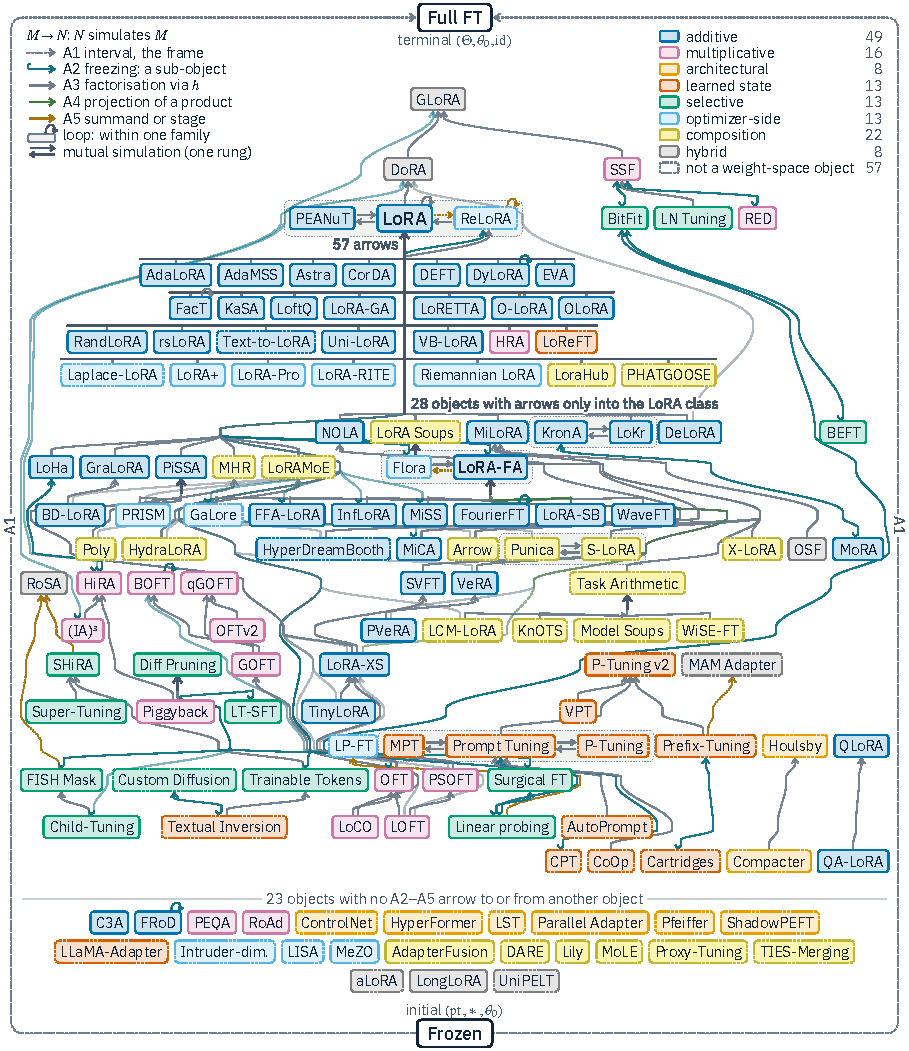
\includegraphics[width=\linewidth]{figures/graph}
\caption{\textbf{The category of core methods.} A layered Hasse diagram (\bgref{A.16}), from Frozen (initial, bottom) to Full FT (terminal, top); the dashed outer frame stands for the A1 arrows Frozen${}\to M\to{}$Full FT of every weight-space method $M$ (\thmref{Observation}{I.4}(a)). Chips are the \nCore{} core methods, coloured by modification kind and dashed for the $57$ that are not objects of the weight-space slice. An arrow $M\to N$ points up and means that $N$ simulates $M$ through a pointed smooth map $h$ with $\rho_N\circ h=\rho_M$ (\thmref{Definition}{I.2}). All $161$ recorded arrows between two core methods are drawn, coloured by rule (Table~\ref{tab:atlas-rules}): $29$ by freezing (A2, hooked tail), $122$ by factorisation (A3), $2$ by products (A4) and $8$ by sums or stages (A5). The $7$ loops land on another member of a family, as $\mathrm{LoRA}_r\to\mathrm{LoRA}_{r+1}$ does, and the $5$ classes of mutually simulating families share a rung in a grey box. Arrows into a method with four or more incoming arrows from outside its class end in one trunk ($57$ into LoRA), and the $28$ methods whose arrows all land in the LoRA class form the comb beneath it. The $26$ lighter arrows are composites, also reached by a longer path of arrows.}\label{fig:graph}
\end{figure}

The atlas is meant to grow. A new method enters by answering the seven questions and exhibiting its arrows, each with its
map $h$; a disputed comparison is settled by an explicit $h$ or by one of the three tests.
